\subsection*{\underline{طراحی UI پروژه}}

در این پروژه ما از تم Material3 استفاده کردیم. برای این در ابتدا Component های مختلف این تم را داخل فیگما جمع‌آوری کردیم و شروع به طراحی UI پروژه کردیم.



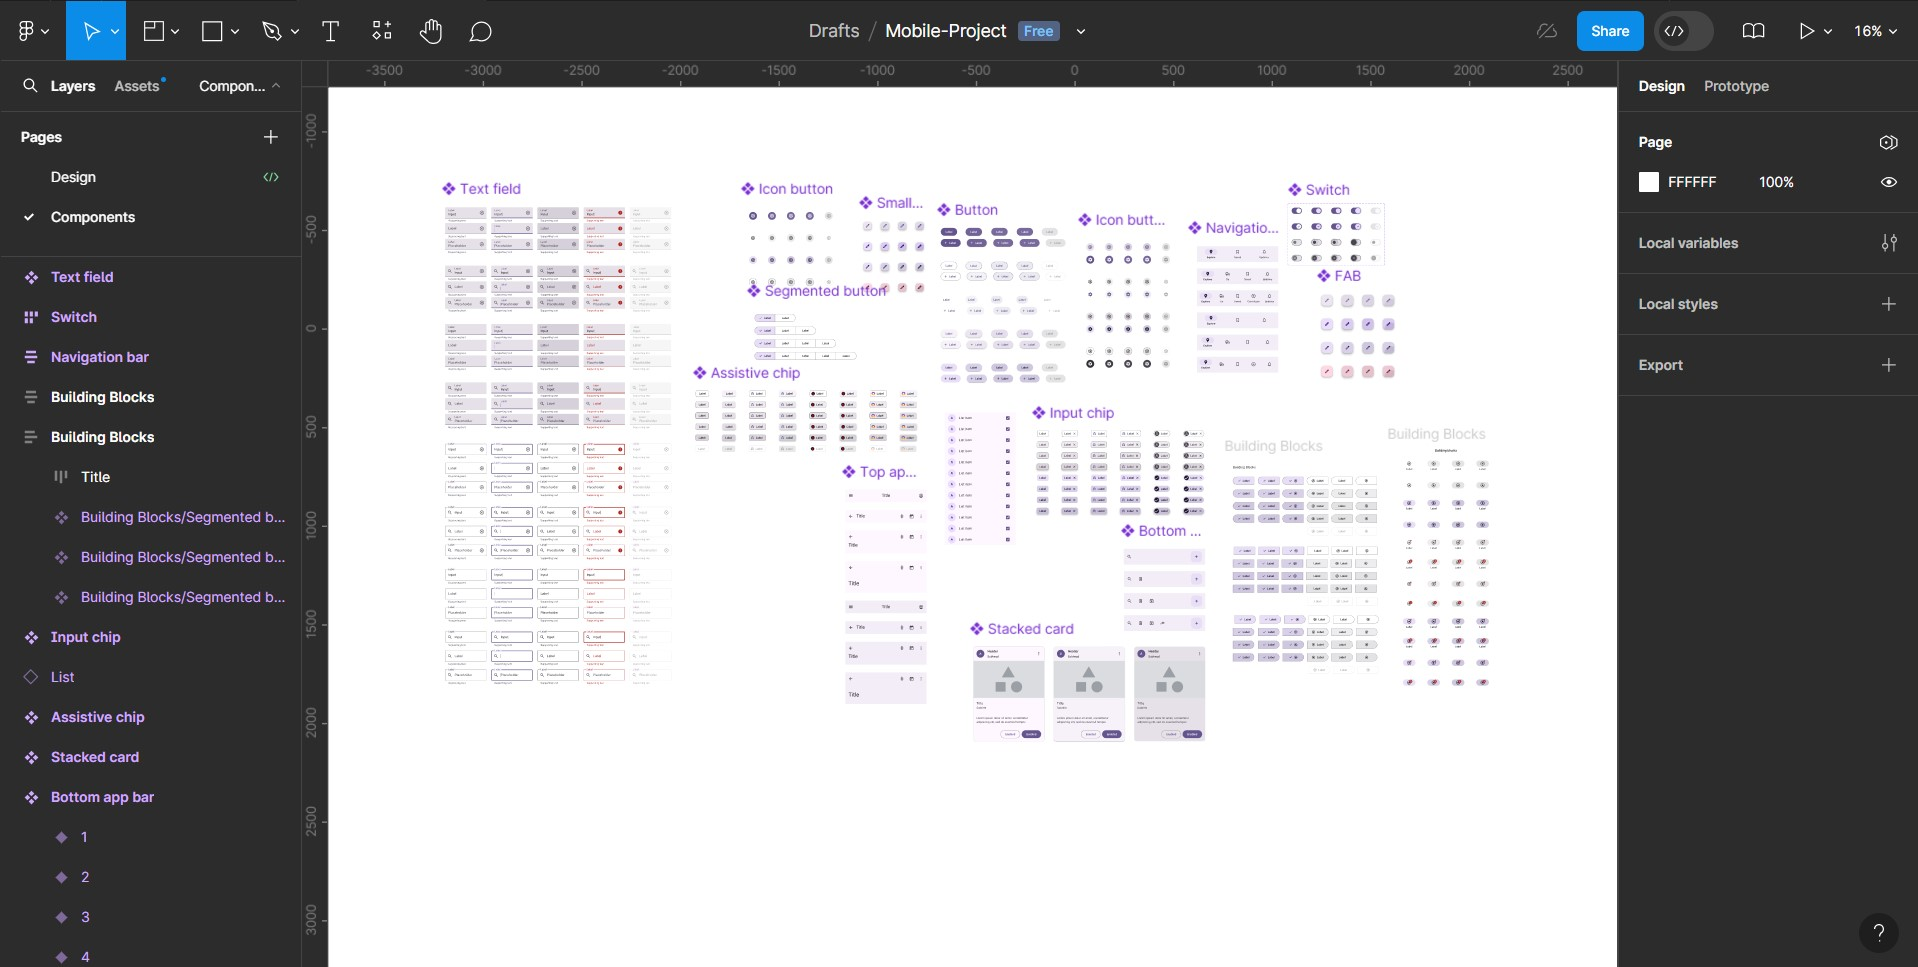
\includegraphics[width=1\linewidth]{figs/1}




پس از آن با توجه به نیازسنجی انجام شده برای بخش های مختلف پروژه، شروع به زدن UI آن کردیم.


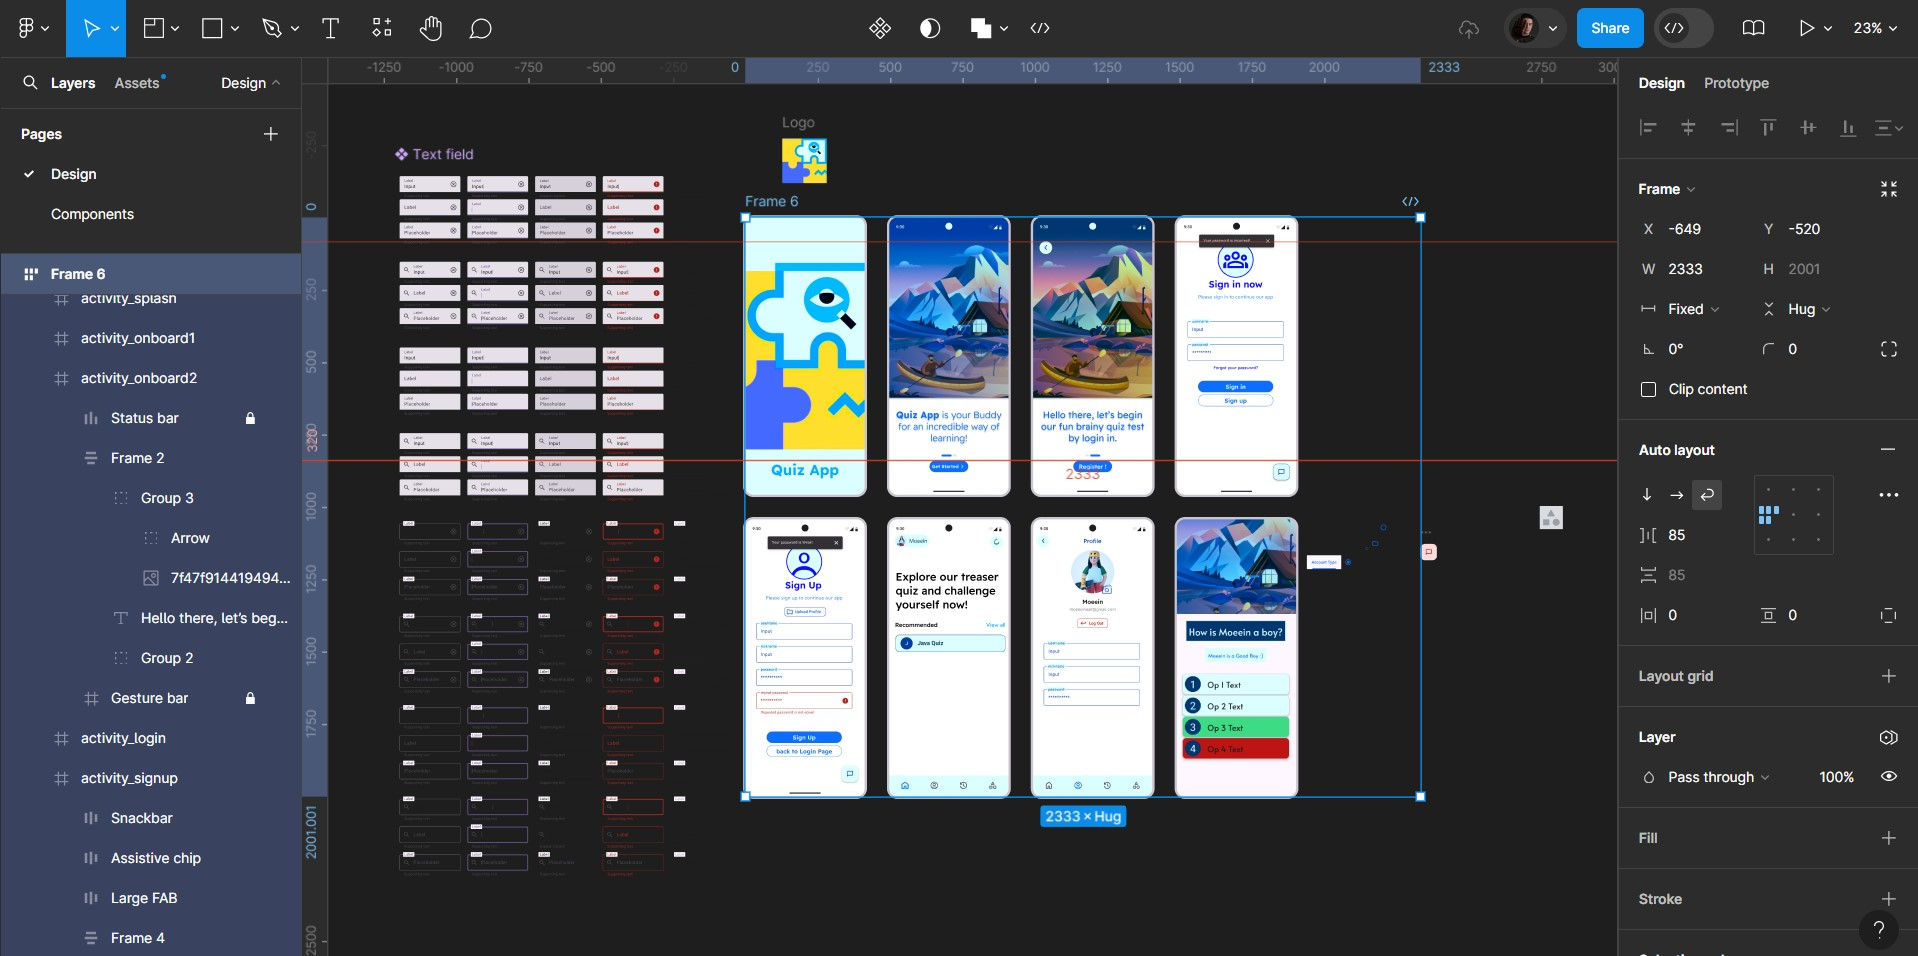
\includegraphics[width=1\linewidth]{figs/2}

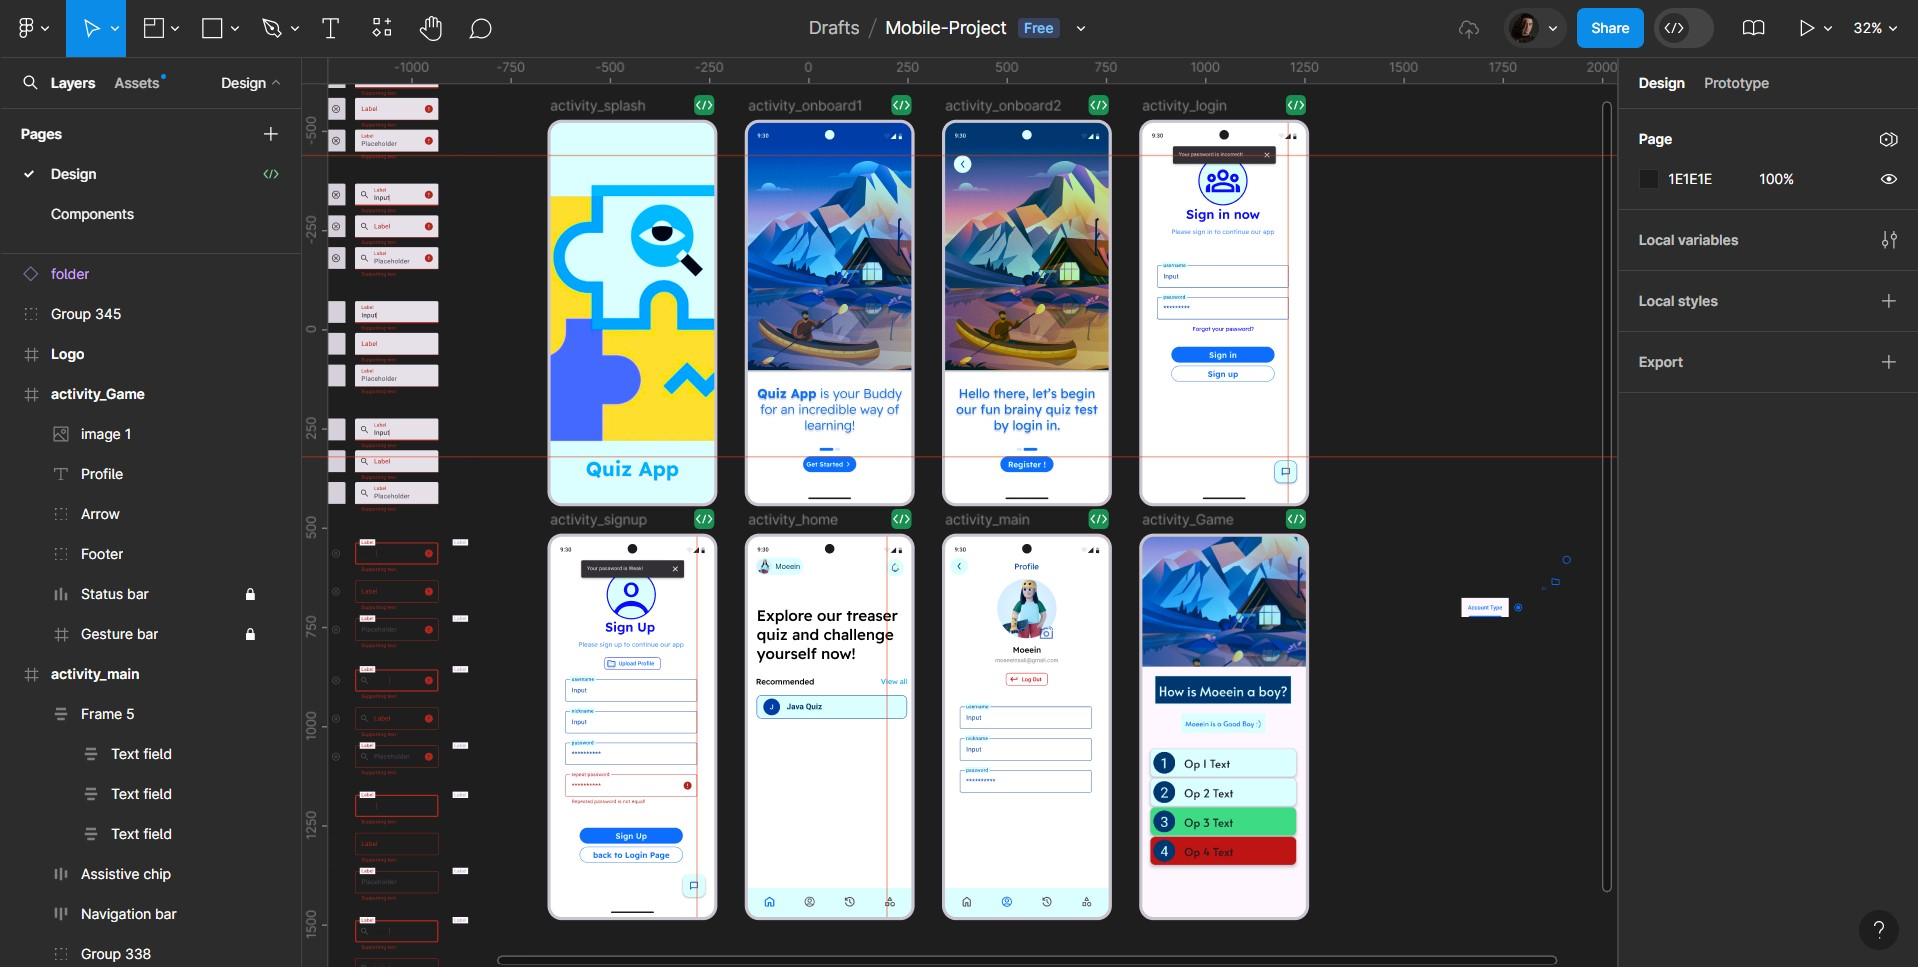
\includegraphics[width=1\linewidth]{figs/3}

در نهایت تم Material3 را به پروژه اضافه کردیم و شروع به استفاده از Component های آن کردیم و فرانت پروژه را زدیم.


دیزاین های ما داخل این پروژه ی فیگما موجود است:
\href{https://www.figma.com/design/SNXPfXCwEaH4mfpgiuE182/Mobile-Project?node-id=0-1&t=ZU7eZkuFNwZp494n-1}{Figma Project}